% Options for packages loaded elsewhere
\PassOptionsToPackage{unicode}{hyperref}
\PassOptionsToPackage{hyphens}{url}
\PassOptionsToPackage{dvipsnames,svgnames*,x11names*}{xcolor}
%
\documentclass[
]{memoir}
\usepackage{amsmath,amssymb}
\usepackage{lmodern}
\usepackage{ifxetex,ifluatex}
\ifnum 0\ifxetex 1\fi\ifluatex 1\fi=0 % if pdftex
  \usepackage[T1]{fontenc}
  \usepackage[utf8]{inputenc}
  \usepackage{textcomp} % provide euro and other symbols
\else % if luatex or xetex
  \usepackage{unicode-math}
  \defaultfontfeatures{Scale=MatchLowercase}
  \defaultfontfeatures[\rmfamily]{Ligatures=TeX,Scale=1}
  \setmonofont[]{Inconsolata}
\fi
% Use upquote if available, for straight quotes in verbatim environments
\IfFileExists{upquote.sty}{\usepackage{upquote}}{}
\IfFileExists{microtype.sty}{% use microtype if available
  \usepackage[]{microtype}
  \UseMicrotypeSet[protrusion]{basicmath} % disable protrusion for tt fonts
}{}
\makeatletter
\@ifundefined{KOMAClassName}{% if non-KOMA class
  \IfFileExists{parskip.sty}{%
    \usepackage{parskip}
  }{% else
    \setlength{\parindent}{0pt}
    \setlength{\parskip}{6pt plus 2pt minus 1pt}}
}{% if KOMA class
  \KOMAoptions{parskip=half}}
\makeatother
\usepackage{xcolor}
\IfFileExists{xurl.sty}{\usepackage{xurl}}{} % add URL line breaks if available
\IfFileExists{bookmark.sty}{\usepackage{bookmark}}{\usepackage{hyperref}}
\hypersetup{
  pdftitle={Data Science per psicologi},
  pdfauthor={Corrado Caudek},
  colorlinks=true,
  linkcolor=Maroon,
  filecolor=Maroon,
  citecolor=Blue,
  urlcolor=Blue,
  pdfcreator={LaTeX via pandoc}}
\urlstyle{same} % disable monospaced font for URLs
\usepackage{color}
\usepackage{fancyvrb}
\newcommand{\VerbBar}{|}
\newcommand{\VERB}{\Verb[commandchars=\\\{\}]}
\DefineVerbatimEnvironment{Highlighting}{Verbatim}{commandchars=\\\{\}}
% Add ',fontsize=\small' for more characters per line
\usepackage{framed}
\definecolor{shadecolor}{RGB}{248,248,248}
\newenvironment{Shaded}{\begin{snugshade}}{\end{snugshade}}
\newcommand{\AlertTok}[1]{\textcolor[rgb]{0.94,0.16,0.16}{#1}}
\newcommand{\AnnotationTok}[1]{\textcolor[rgb]{0.56,0.35,0.01}{\textbf{\textit{#1}}}}
\newcommand{\AttributeTok}[1]{\textcolor[rgb]{0.77,0.63,0.00}{#1}}
\newcommand{\BaseNTok}[1]{\textcolor[rgb]{0.00,0.00,0.81}{#1}}
\newcommand{\BuiltInTok}[1]{#1}
\newcommand{\CharTok}[1]{\textcolor[rgb]{0.31,0.60,0.02}{#1}}
\newcommand{\CommentTok}[1]{\textcolor[rgb]{0.56,0.35,0.01}{\textit{#1}}}
\newcommand{\CommentVarTok}[1]{\textcolor[rgb]{0.56,0.35,0.01}{\textbf{\textit{#1}}}}
\newcommand{\ConstantTok}[1]{\textcolor[rgb]{0.00,0.00,0.00}{#1}}
\newcommand{\ControlFlowTok}[1]{\textcolor[rgb]{0.13,0.29,0.53}{\textbf{#1}}}
\newcommand{\DataTypeTok}[1]{\textcolor[rgb]{0.13,0.29,0.53}{#1}}
\newcommand{\DecValTok}[1]{\textcolor[rgb]{0.00,0.00,0.81}{#1}}
\newcommand{\DocumentationTok}[1]{\textcolor[rgb]{0.56,0.35,0.01}{\textbf{\textit{#1}}}}
\newcommand{\ErrorTok}[1]{\textcolor[rgb]{0.64,0.00,0.00}{\textbf{#1}}}
\newcommand{\ExtensionTok}[1]{#1}
\newcommand{\FloatTok}[1]{\textcolor[rgb]{0.00,0.00,0.81}{#1}}
\newcommand{\FunctionTok}[1]{\textcolor[rgb]{0.00,0.00,0.00}{#1}}
\newcommand{\ImportTok}[1]{#1}
\newcommand{\InformationTok}[1]{\textcolor[rgb]{0.56,0.35,0.01}{\textbf{\textit{#1}}}}
\newcommand{\KeywordTok}[1]{\textcolor[rgb]{0.13,0.29,0.53}{\textbf{#1}}}
\newcommand{\NormalTok}[1]{#1}
\newcommand{\OperatorTok}[1]{\textcolor[rgb]{0.81,0.36,0.00}{\textbf{#1}}}
\newcommand{\OtherTok}[1]{\textcolor[rgb]{0.56,0.35,0.01}{#1}}
\newcommand{\PreprocessorTok}[1]{\textcolor[rgb]{0.56,0.35,0.01}{\textit{#1}}}
\newcommand{\RegionMarkerTok}[1]{#1}
\newcommand{\SpecialCharTok}[1]{\textcolor[rgb]{0.00,0.00,0.00}{#1}}
\newcommand{\SpecialStringTok}[1]{\textcolor[rgb]{0.31,0.60,0.02}{#1}}
\newcommand{\StringTok}[1]{\textcolor[rgb]{0.31,0.60,0.02}{#1}}
\newcommand{\VariableTok}[1]{\textcolor[rgb]{0.00,0.00,0.00}{#1}}
\newcommand{\VerbatimStringTok}[1]{\textcolor[rgb]{0.31,0.60,0.02}{#1}}
\newcommand{\WarningTok}[1]{\textcolor[rgb]{0.56,0.35,0.01}{\textbf{\textit{#1}}}}
\usepackage{longtable,booktabs,array}
\usepackage{calc} % for calculating minipage widths
% Correct order of tables after \paragraph or \subparagraph
\usepackage{etoolbox}
\makeatletter
\patchcmd\longtable{\par}{\if@noskipsec\mbox{}\fi\par}{}{}
\makeatother
% Allow footnotes in longtable head/foot
\IfFileExists{footnotehyper.sty}{\usepackage{footnotehyper}}{\usepackage{footnote}}
\makesavenoteenv{longtable}
\usepackage{graphicx}
\makeatletter
\def\maxwidth{\ifdim\Gin@nat@width>\linewidth\linewidth\else\Gin@nat@width\fi}
\def\maxheight{\ifdim\Gin@nat@height>\textheight\textheight\else\Gin@nat@height\fi}
\makeatother
% Scale images if necessary, so that they will not overflow the page
% margins by default, and it is still possible to overwrite the defaults
% using explicit options in \includegraphics[width, height, ...]{}
\setkeys{Gin}{width=\maxwidth,height=\maxheight,keepaspectratio}
% Set default figure placement to htbp
\makeatletter
\def\fps@figure{htbp}
\makeatother
\setlength{\emergencystretch}{3em} % prevent overfull lines
\providecommand{\tightlist}{%
  \setlength{\itemsep}{0pt}\setlength{\parskip}{0pt}}
\setcounter{secnumdepth}{5}
\chapterstyle{bianchi}

\usepackage{amsmath}
\usepackage[italian]{babel} 
\usepackage{lmodern} 
\usepackage{booktabs}
\usepackage{hyperref}
\hypersetup{
  colorlinks=true
}
\usepackage[
  labelfont=bf, 
  font={small, it} 
]{caption} 
\usepackage{upquote} % print correct quotes in verbatim-environments
\usepackage[autostyle, italian=quotes]{csquotes}
\usepackage{xfrac}

\raggedbottom % allow variable (ragged) site heights
\frenchspacing
\setlength\parskip{1.5pt plus 1pt minus 0.5pt}

\DeclareMathOperator{\Var}{Var} % Define variance operator
\DeclareMathOperator{\SD}{SD} % Define sd operator
\DeclareMathOperator{\Cov}{Cov} % Define covariance operator
\DeclareMathOperator{\Corr}{Corr} % Define correlation operator
\DeclareMathOperator{\Me}{Me} % Define mediane operator
\DeclareMathOperator{\Mo}{Mo} % Define mode operator
\DeclareMathOperator{\Bin}{Bin} % Define binomial operator
\DeclareMathOperator{\Cauchy}{Cauchy} % Define Cauchy operator
\DeclareMathOperator{\B}{\mathscr{B}} % Define Bernoulli operator
\newcommand{\R}{\textsf{R}} % Define R programming language symbol
\newcommand{\E}{\mathbb{E}} % Define expected value operator
\newcommand{\Real}{\mathbb{R}} % Define real number operator
\newcommand{\Prob}{\mathscr{P}}
\DeclareMathOperator*{\argmin}{arg\,min} % thin space, limits on side in displays
\DeclareMathOperator*{\argmax}{arg\,max} % thin space, limits on side in displays

\usepackage{microtype}

\ifluatex
  \usepackage{selnolig}  % disable illegal ligatures
\fi
\usepackage[]{natbib}
\bibliographystyle{apalike}

\title{Data Science per psicologi}
\author{Corrado Caudek}
\date{2021-09-13}

\usepackage{amsthm}
\newtheorem{theorem}{Teorema}[chapter]
\newtheorem{lemma}{Lemma}[chapter]
\newtheorem{corollary}{Corollario}[chapter]
\newtheorem{proposition}{Proposizione}[chapter]
\newtheorem{conjecture}{Congettura}[chapter]
\theoremstyle{definition}
\newtheorem{definition}{Definizione}[chapter]
\theoremstyle{definition}
\newtheorem{example}{Esempio}[chapter]
\theoremstyle{definition}
\newtheorem{exercise}{Exercizio}[chapter]
\theoremstyle{definition}
\newtheorem{hypothesis}{Hypothesis}[chapter]
\theoremstyle{remark}
\newtheorem*{remark}{Osservazione}
\newtheorem*{solution}{Soluzione}
\begin{document}
\maketitle

{
\hypersetup{linkcolor=}
\setcounter{tocdepth}{1}
\tableofcontents
}
\newpage

\vspace*{5cm}

\thispagestyle{empty}

\hypertarget{part-verosimiglianza}{%
\part*{Verosimiglianza}\label{part-verosimiglianza}}
\addcontentsline{toc}{part}{Verosimiglianza}

\hypertarget{la-funzione-di-verosimiglianza}{%
\chapter{La funzione di verosimiglianza}\label{la-funzione-di-verosimiglianza}}

Per introdurre la funzione di verosimiglianza utilizzeremo un esempio proposto da \citet{McElreath_rethinking}.\footnote{Per una trattazione più formale, si consulti il tutorial di \citet{etz2018introduction}.} Supponiamo di tenere in mano un mappamondo e di chiederci: ``qual'è la proporzione della superficie terreste ricoperta d'acqua?'' Sembra una domanda a cui è difficile rispondere. Ma \citet{McElreath_rethinking} propone questa idea brillante: lanciamo in aria il mappamondo e, quando lo riprendiamo, osserviamo se la superfice del mappamondo sotto il nostro dito indice destro rappresenta acqua o terra. Possiamo ripetere questa procedura più volte, così da ottenere un campione causale di diverse porzioni della superficie dal mappamondo. Eseguiamo l'esperimento casuale nove volte e osserviamo i seguenti risultati: A, T, A, A, A, T, A, T, A, dove ``A'' indica acqua e ``T'' indica terra.

\hypertarget{dati-e-parametri}{%
\section{Dati e parametri}\label{dati-e-parametri}}

Per l'esempio del mappamondo possiamo dire quanto segue:

\begin{enumerate}
\def\labelenumi{\arabic{enumi}.}
\tightlist
\item
  la proporzione del pianeta Terra ricoperta d'acqua è \(\theta\);
\item
  un singolo lancio del mappamondo ha una probabilità \(\theta\) di produrre l'osservazione ``acqua'' (A);
\item
  i lanci del mappamondo sono indipendenti (nel senso che il risultato
  di un lancio non influenza i risultati degli altri lanci).
\end{enumerate}

Nella descrizione precedente, i \emph{dati} sono le frequenze degli eventi \(A\) (``acqua'') e \(T\) (``terra'') prodotte da una serie di osservazioni. La somma delle frequenze di \(A\) e \(T\) è il numero totale dei lanci del mappamondo: \(N = A + T\). Oltre ai dati, abbiamo anche fatto riferimento alla proporzione (incognita) di acqua sul globo terrestre. Tale proporzione corrisponde al \emph{parametro} \(\theta \in \Theta\), dove \(\Theta\) rappresenta lo spazio parametrico in cui può variare il parametro \(\theta\). Nel caso presente, \(\theta \in [0, 1]\), in quanto \(\theta\) è una proporzione. La descrizione del parametro \(\theta\) rappresenta l'obiettivo dell'inferenza.

Anche se il parametro \(\theta\) non può essere direttamente osservato è possibile inferire il suo valore a partire dai dati. Avendo specificato ciò che abbiamo detto sopra, possiamo formulare un \emph{modello statistico}: abbiamo una sequenza di prove Bernoulliane indipendenti e, dunque, il modello statistico sarà quello binomiale. Prima di descrivere questo modello in dettaglio, è utile visualizzare il suo comportamento. Dopo aver visto come questo modello apprende dai dati ci porremo il problema di capire come funziona.

\hypertarget{come-impara-un-modello-statistico}{%
\subsection{Come impara un modello statistico?}\label{come-impara-un-modello-statistico}}

Prima di lanciare in aria il mappamondo e di ottenere il primo dato, non sappiamo nulla del parametro \(\theta\). Dato che \(\theta\) è una proporzione, i suoi valori possibili vanno da 0 a 1. Se non possediamo alcuna informazione su \(\theta\), allora riteniamo che tutti i valori \(\theta\) siano egualmente credibili. Rappresentiamo dunque la nostra incertezza a proposito del parametro \(\theta\) mediante una distribuzione uniforme su tutti i valori \(\theta\), come indicato dalla linea tratteggiata nel pannello \(n = 1\) della figura \ref{fig:rethinkingmodlearn}.

\begin{figure}

{\centering 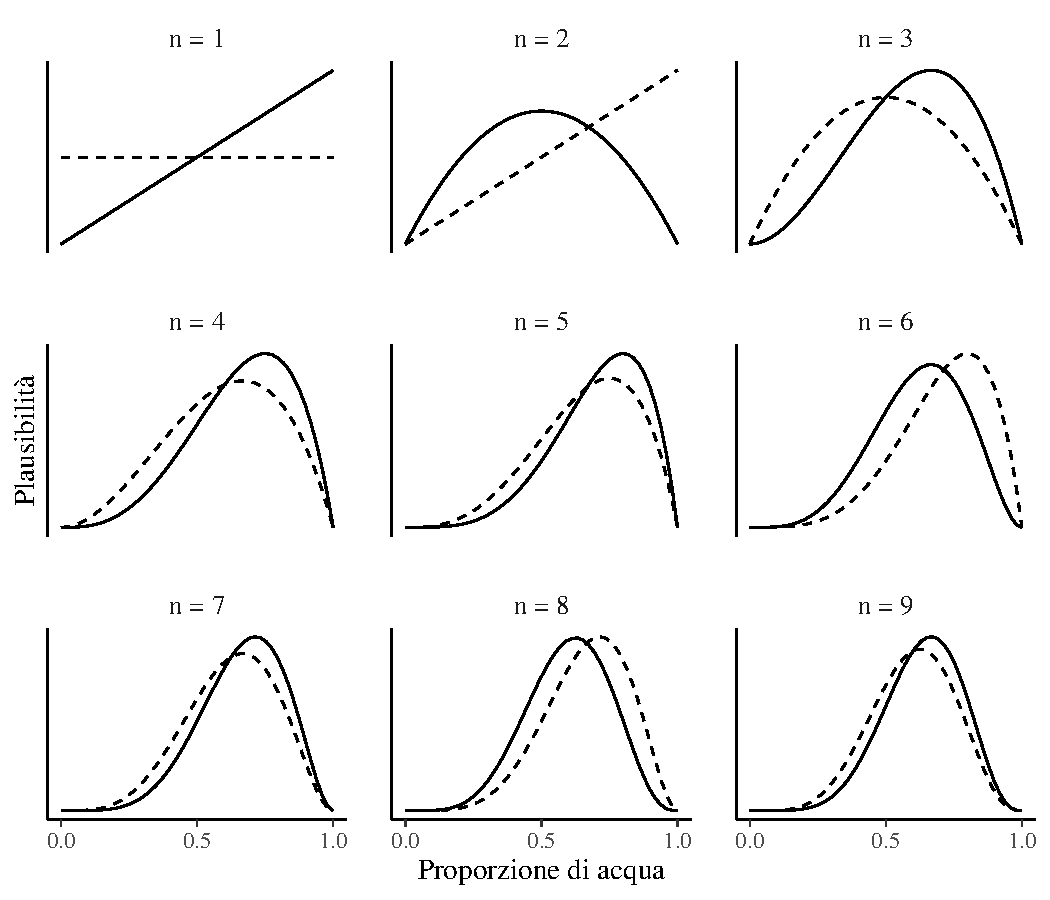
\includegraphics[width=1\linewidth]{images/rethinking_fig_2_5} 

}

\caption{Come un modello statistico impara? Ciascun lancio del mappamondo produce un'osservazione: acqua (A) o terra (T). La stima della proporzione di acqua ($\theta$) sulla superficie terreste prodotta dal modello è espressa nei termini del grado di credibilità (o Plausibilità, nella figura) di ciascun possibile valore $\theta$. Le linee e le curve nella figura rappresentano il grado di credibilità dei valori $\theta$ per diversi set di dati. In ogni pannello, le credibilità (curva tratteggiata) calcolate in base alle informazioni fornite dai lanci $1, \dots, k$ vengono aggiornate a seguito dell'informazione fornita dal lancio $k + 1$. I nuovi valori di credibilità di $\theta$ sono rappresentati dalla curva solida.}\label{fig:rethinkingmodlearn}
\end{figure}

Lanciamo in aria il mappamondo una prima volta e, quando lo riprendiamo, notiamo che sotto il nostro indice destro c'è ``acqua''. Dopo avere osservato il risultato del primo lancio, ovvero ``A'', il modello aggiorna le credibilità dei valori del parametro \(\theta\) che ora sono rappresentate dalla linea continua nel pannello \(n = 1\) della figura \ref{fig:rethinkingmodlearn}. La credibilità associata all'evento \(\theta = 0\) è scesa esattamente a zero, l'equivalente di ``impossibile''. Infatti, avendo osservato almeno un luogo sul mappamondo in cui c'è dell'acqua, possiamo dire che l'evento ``non c'è acqua'' (ovvero \(\theta = 0\)) è impossibile. Allo stesso modo, la credibilità di \(\theta > 0.5\) è aumentata. Non abbiamo ancora evidenze che ci sia terra sul mappamondo, quindi le credibilità iniziali sono state modificate per essere coerenti con questa informazione: le credibilità associate a \(\theta\) aumentano passando dal valore \(\theta = 0\) a valore \(\theta = 1\), in maniera coerente con i dati che abbiamo. Il punto importante è che le evidenze disponibili fino a questo momento vengono incorporata nelle credibilità attribuite a ciascun possibile valore \(\theta\). Il modello implementa questa logica in maniera \emph{automatica}. Non è necessario fornire al modello alcuna istruzione per ottenere questo risultato. La teoria della probabilità svolge tutti i
calcoli necessari per noi.

Lanciamo in aria il mappamondo una seconda volta e osserviamo ``T''. Consideriamo dunque il pannello \emph{n = 2} della figura \ref{fig:rethinkingmodlearn}. La linea tratteggiata in questo pannello ricopia semplicemente la descrizione del livello di credibilità di ciascun valore \(\theta\) che era disponibile nel caso di un solo lancio del mappamondo. La linea continua, invece, aggiorna tali valori di credibilità incorporando l'informazione secondo la quale in due lanci abbiamo ottenuto ``acqua'' una volta e ``terra'' una volta. Vediamo che ora il valore di credibilità di \(\theta\) è uguale a zero per l'evento \(\theta = 0\); infatti, abbiamo osservato ``acqua'' nel primo lancio. In maniera corrispondente, il valore di credibilità di \(\theta\) è uguale a zero per l'evento \(\theta = 1\) (c'è solo acqua); infatti, abbiamo osservato ``terra'' nel secondo lancio. Avendo osservato ``acqua'' nel 50\% dei casi, il valore più verosimile per \(\theta\) sarà 0.5, come indicato dalla linea continua in questo pannello.

Nei pannelli rimanenti della figura \ref{fig:rethinkingmodlearn} i nuovi dati prodotti dai successivi lanci del mappamondo vengono analizzati dal modello, uno alla volta. La curva tratteggiata in ciascun pannello corrisponde alla curva solida del pannello precedente, spostandosi da sinistra a destra e dall'alto verso il basso. Ogni volta che si ottiene un dato \emph{A} il picco della curva di credibilità si sposta a destra, verso valori più grandi di \(\theta\). Ogni volta si ottiene \emph{T} ci si sposta nella direzione opposta. L'altezza massima della curva aumenta con ogni campione, il che significa che, all'aumentare della quantità di prove, viene associato un livello di credibilità maggiore ad un minor numero di valori di \(\theta\). Man mano che viene aggiunta una nuova osservazione, la curva che rappresenta la credibilità dei valori \(\theta\) viene aggiornata in maniera coerente con tutte le osservazioni precedenti.

\hypertarget{la-funzione-di-verosimiglianza-1}{%
\section{La funzione di verosimiglianza}\label{la-funzione-di-verosimiglianza-1}}

Nella figura \ref{fig:rethinkingmodlearn} abbiamo descritto con una curva il grado di credibilità associato a ciascun valore del parametro \(\theta\). Una curva è il grafico di una funzione matematica. In statistica, tale funzione si chiama \emph{verosimiglianza} di \(\theta\) basata sui dati \(y = (y_1, \dots, y_n)\).

\hypertarget{la-verosimiglianza-del-modello-binomiale}{%
\subsection{La verosimiglianza del modello binomiale}\label{la-verosimiglianza-del-modello-binomiale}}

Vediamo ora come si costruisce la funzione di verosimiglianza per l'esperimento casuale corrispondente al lancio del mappamondo. Gli eventi possibili che possono essere osservati nell'esperimento casuale sono acqua (\(A\)) e terra (\(T\)). Avendo lanciato in aria il mappamondo 9 volte, abbiamo osservato una serie di eventi \(A\) e \(T\). Ora ci chiediamo: qual è la probabilità di osservare questo \emph{specifico} campione (6 volte ``acqua'' in 9 lanci del mappamondo) nell'universo di tutte le possibili sequenze risultanti da 9 lanci del mappamondo? Sembra una domanda a cui è molto difficile rispondere, ma in realtà non è vero. Se specifichiamo le caratteristiche dell'esperimento casuale come abbiamo fatto sopra, ovvero: (1) ogni lancio è indipendente dagli altri e (2) la probabilità di osservare ``acqua'' è la stessa in ciascun lancio, allora la teoria della probabilità ci consente di trovare facilmente una risposta alla nostra domanda. Le caratteristiche dell'esperimento casuale che abbiamo descritto specificano infatti una variabile casuale binomiale. La funzione che stiamo cercando, dunque, è la distribuzione binomiale. In precedenza abbiamo discusso tale distribuzione facendo riferimento al lancio di una moneta. Ma l'esperimento casuale corrispondente a \(n\) lanci di una moneta è strutturalmente identico a quello del mappamondo (gli unici esiti possibili sono ``acqua'' e ``terra'', i lanci sono indipendenti gli uni dagli altri e la probabilità di osservare ``acqua'' rimane costante in ciascun lancio). Possiamo dunque usare la distribuzione binomiale per descrivere la probabilità di osservare \emph{A} = ``numero di volte in cui abbiamo osservato acqua'' e \emph{T} = ``numero di volte in cui abbiamo osservato terra'', quando il nostro mappamondo è stato lanciato in aria per \emph{n = A + T} volte. Tale probabilità è data dalla distribuzione binomiale di parametro \(\theta\):

\begin{equation}
P(A, T \mid \theta) = \frac{(A + T)!}{A!T!} \theta^A + (1-\theta)^T.
\label{eq:binomwater}
\end{equation}

In altre parole, la frequenza degli eventi ``numero di volte in cui abbiamo osservato acqua'' e ``numero di volte in cui abbiamo osservato terra'' segue la distribuzione binomiale nella quale la probabilità di osservare ``acqua'' in ciascun lancio è uguale a \(\theta\).

\hypertarget{la-verosimiglianza-vista-da-vicino}{%
\subsection{La verosimiglianza vista da vicino}\label{la-verosimiglianza-vista-da-vicino}}

Ma cosa dobbiamo fare, in pratica, per generare le funzioni di verosimiglianza che sono rappresentate nei diversi pannelli della figura \ref{fig:rethinkingmodlearn}? Iniziamo con una definizione formale.

\begin{definition}
La \emph{funzione di verosimiglianza} \(\mathcal{L}(\theta \mid y) = f(y \mid \theta), \theta \in \Theta,\) è la funzione di massa o di densità di probabilità dei dati \(y\) vista come una funzione del parametro sconosciuto \(\theta\).
\end{definition}

Spesso per indicare la verosimiglianza si scrive \(\mathcal{L}(\theta)\) se è chiaro a quali valori \(y\) ci si riferisce. La verosimiglianza \(\mathcal{L}\) è una curva (in generale, una superficie) nello spazio \(\Theta\) del parametro (in generale, dei parametri \(\boldsymbol\theta\)) che riflette la credibilità relativa dei valori \(\theta\) alla luce dei dati osservati. Notiamo un punto importante: la funzione \(\mathcal{L}(\theta \mid y)\) non è una funzione di densità. Infatti, essa non racchiude un'area unitaria.

Nel caso presente, la funzione di verosimiglianza è descritta dalla \eqref{eq:binomwater}, ovvero, corrisponde alla funzione binomiale di parametro \(\theta \in (0, 1)\) sconosciuto. Nell'esempio che stiamo discutendo, abbiamo osservato ``acqua'' sei volte in nove lanci del mappamondo. Dunque, \(y = 6\) successi in \(n = 9\) prove. Per i dati del campione considerato, la funzione di verosimiglianza diventa

\begin{equation}
\mathcal{L}(\theta \mid y) = \frac{(6 + 3)!}{6!3!} \theta^6 + (1-\theta)^3.
\label{eq:likebino69}
\end{equation}

La definizione precedente ci dice che, per costruire la funzione di verosimiglianza, dobbiamo applicare tante volte la \eqref{eq:likebino69} \emph{tenendo costanti i dati} e cambiando ogni volta il valore \(\theta\).

Per esempio, se poniamo \(\theta = 0.1\)

\[
\mathcal{L}(\theta \mid y) = \frac{(6 + 3)!}{6!3!} 0.1^6 + (1-0.1)^3
\]

otteniamo il valore 0.0446. Se poniamo \(\theta = 0.2\)

\[
\mathcal{L}(\theta \mid y) = \frac{(6 + 3)!}{6!3!} 0.2^6 + (1-0.2)^3
\]

otteniamo 0.1762; e così via.

La tabella seguente riportata alcuni valori rappresentativi della funzione di verosimiglianza definita da 6 successi in 9 prove Bernoulliane.

\hypertarget{tab:likebino}{}
\begin{longtable}[]{@{}cc@{}}
\toprule
\(\theta\) & \(\mathcal{L}(\theta \mid y)\) \\
\midrule
\endhead
0.0 & 0.0000 \\
0.1 & 0.0001 \\
0.2 & 0.0028 \\
0.3 & 0.0210 \\
0.4 & 0.0743 \\
0.5 & 0.1641 \\
0.6 & 0.2508 \\
0.7 & 0.2668 \\
0.8 & 0.1762 \\
0.9 & 0.0446 \\
1.0 & 0.0000 \\
\bottomrule
\end{longtable}

La figura \ref{fig:likelihoodwater} fornisce una rappresentazione grafica della funzione di verosimiglianza -- la figura è stata costruita utilizzando 100 valori equispaziati \(\theta \in [0, 1]\).

\begin{Shaded}
\begin{Highlighting}[]
\NormalTok{n }\OtherTok{\textless{}{-}} \DecValTok{9}
\NormalTok{y }\OtherTok{\textless{}{-}} \DecValTok{6}
\NormalTok{theta }\OtherTok{\textless{}{-}} \FunctionTok{seq}\NormalTok{(}\DecValTok{0}\NormalTok{, }\DecValTok{1}\NormalTok{, }\AttributeTok{length.out=}\DecValTok{100}\NormalTok{)}
\NormalTok{like }\OtherTok{\textless{}{-}} \FunctionTok{choose}\NormalTok{(n, y) }\SpecialCharTok{*}\NormalTok{ theta}\SpecialCharTok{\^{}}\NormalTok{y }\SpecialCharTok{*}\NormalTok{ (}\DecValTok{1} \SpecialCharTok{{-}}\NormalTok{ theta)}\SpecialCharTok{\^{}}\NormalTok{(n }\SpecialCharTok{{-}}\NormalTok{ y)}
\FunctionTok{plot}\NormalTok{(}
\NormalTok{  theta, like, }
  \AttributeTok{type =} \StringTok{\textquotesingle{}l\textquotesingle{}}\NormalTok{, }
  \AttributeTok{xaxt =} \StringTok{"n"}\NormalTok{, }
  \AttributeTok{bty =} \StringTok{\textquotesingle{}l\textquotesingle{}}\NormalTok{,}
  \AttributeTok{main =} \StringTok{"Funzione di verosimiglianza"}\NormalTok{, }
  \AttributeTok{ylab =} \FunctionTok{expression}\NormalTok{(}\FunctionTok{L}\NormalTok{(theta)),}
  \AttributeTok{xlab =} \FunctionTok{expression}\NormalTok{(}\StringTok{\textquotesingle{}Valori possibili di\textquotesingle{}} \SpecialCharTok{\textasciitilde{}}\NormalTok{ theta)}
\NormalTok{)}
\FunctionTok{axis}\NormalTok{(}\AttributeTok{side =} \DecValTok{1}\NormalTok{, }\AttributeTok{at =} \FunctionTok{seq}\NormalTok{(}\DecValTok{0}\NormalTok{, }\DecValTok{1}\NormalTok{, }\AttributeTok{length.out =} \DecValTok{11}\NormalTok{))}
\FunctionTok{segments}\NormalTok{(}
  \FloatTok{0.67}\NormalTok{, }\DecValTok{0}\NormalTok{, }\FloatTok{0.67}\NormalTok{, }
  \FunctionTok{choose}\NormalTok{(n, y) }\SpecialCharTok{*} \FloatTok{0.67}\SpecialCharTok{\^{}}\NormalTok{y }\SpecialCharTok{*}\NormalTok{ (}\DecValTok{1} \SpecialCharTok{{-}} \FloatTok{0.67}\NormalTok{)}\SpecialCharTok{\^{}}\NormalTok{(n }\SpecialCharTok{{-}}\NormalTok{ y), }
  \AttributeTok{lty =} \DecValTok{2}
\NormalTok{)}
\end{Highlighting}
\end{Shaded}

\begin{figure}

{\centering 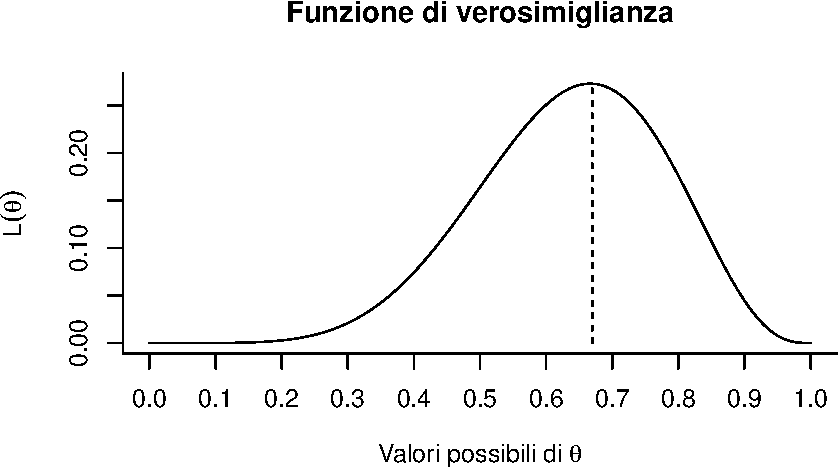
\includegraphics{024_likelihood_files/figure-latex/likelihoodwater-1} 

}

\caption{Funzione di verosimiglianza nel caso in cui l'esito acqua sia stato osservato 6 volte in 9 lanci del mappamondo.}\label{fig:likelihoodwater}
\end{figure}

\hypertarget{interpretazione}{%
\subsubsection{Interpretazione}\label{interpretazione}}

Come possiamo interpretare la curva che abbiamo ottenuto? Per alcuni valori \(\theta\) la funzione di verosimiglianza assume valori piccoli; per altri valori \(\theta\) la funzione di verosimiglianza assume valori più grandi. Questi ultimi sono i valori di \(\theta\) ``più credibili'' e il valore 0.67 è il valore più credibile di tutti. In termini più formali possiamo dire che la funzione di verosimiglianza ha la seguente interpretazione: sulla base dei dati, \(\theta_1 \in \Theta\) è più credibile di \(\theta_2 \in \Theta\) come indice del modello probabilistico generatore delle osservazioni se \(\mathcal{L}(\theta_1) > \mathcal{L}(\theta_1)\).

In conclusione, la funzione di verosimiglianza descrive in termini relativi il sostegno empirico che \(\theta \in \Theta\) riceve da \(y\). La figura \ref{fig:rethinkingmodlearn}, infatti, mostra come la funzione di verosimiglianza assume una forma diversa quando \(y\) varia: le curve nei pannelli della figura \ref{fig:rethinkingmodlearn} sono tutte state ottenute usando la \eqref{eq:binomwater}, ma sono tra loro diverse perché i dati sono diversi: 1 successo in 1 prova (abbiamo lanciato il mappamondo una volta e abbiamo osservato ``acqua''); 1 successo in 2 prove (abbiamo lanciato il mappamondo due volte e abbiamo osservato ``acqua'' e ``terra''); 2 successi in 3 prove (abbiamo lanciato il mappamondo tre volte e abbiamo osservato ``acqua'', ``terra'' e ``acqua''); eccetera.

\hypertarget{la-stima-di-massima-verosimiglianza}{%
\subsection{La stima di massima verosimiglianza}\label{la-stima-di-massima-verosimiglianza}}

La funzione di verosimiglianza rappresenta la ``credibilità relativa'' dei valori del parametro di interesse. Ma qual è il valore più credibile? Se utilizziamo soltanto la funzione di verosimiglianza, allora la risposta è data dalla stima di massima verosimiglinza.

\begin{definition}
Un valore di \(\theta\) che massimizza \(\mathcal{L}(\theta \mid y)\) sullo spazio parametrico \(\Theta\) è detto \emph{stima di massima verosimiglinza} (s.m.v.) di \(\theta\) ed è indicato con \(\hat{\theta}\):

\begin{equation}
\hat{\theta} = \text{argmax}_{\theta \in \Theta} \mathcal{L}(\theta).
\end{equation}
\end{definition}

Il paradigma frequentista utilizza la funzione di verosimiglianza quale unico strumento per giungere alla stima del valore più credibile del parametro sconosciuto \(\theta\). Tale stima corrisponde al punto di massimo della funzione di verosimiglianza. Nell'esempio presente, \(\hat{\theta} = 0.6667\). Il massimo della funzione di verosimiglianza, ovvero \(\hat{\theta}\), si può ottenere con metodi numerici o grafici.

In base all'approccio bayesiano, invece, il valore più credibile del parametro sconosciuto \(\theta\) non corrisponde alla s.m.v.. Per l'approccio bayesiano, invece, il valore più credibile del parametro sconosciuto \(\theta\) è dato dalla moda (o media, o mediana) della distribuzione a posteriori \(p(\theta \mid y)\) che si ottiene combinando la verosimiglianza \(p(y \mid \theta)\) con la distribuzione a priori \(p(\theta)\).

\hypertarget{la-log-verosimiglianza}{%
\subsection{La log-verosimiglianza}\label{la-log-verosimiglianza}}

Dal punto di vista pratico risulta più conveniente utilizzare, al posto della funzione di verosimiglianza, il suo logaritmo naturale, ovvero la funzione di log-verosimiglianza

\begin{equation}
\ell(\theta) = \log \mathcal{L}(\theta).\notag
\end{equation}

Poiché il logaritmo è una funzione strettamente crescente (usualmente si considera il logaritmo naturale), allora \(\mathcal{L}(\theta)\) e \(\ell(\theta)\) assumono il massimo (o i punti di massimo) in corrispondenza degli stessi valori di \(\theta\):

\[
\hat{\theta} = \text{argmax}_{\theta \in \Theta} \ell(\theta).
\]

Per le proprietà del logaritmo, si ha

\begin{equation}
\ell(\theta) = \log \left( \prod_{i = 1}^n f(y \mid \theta) \right) = \sum_{i = 1}^n \log f(y \mid \theta).
\end{equation}

Si noti che non è necessario lavorare con i logaritmi, anche se è fortemente consigliato, e questo perché i valori della verosimiglianza, in cui si moltiplicano valori di probabilità molto piccoli, possono diventare estremamente piccoli (qualcosa come \(10^{-34}\)). In tali circostanze, non è sorprendente che i programmi dei computer mostrino problemi di arrotondamento numerico. Le trasformazioni logaritmiche risolvono questo problema.

\hypertarget{derivation-smv-prop}{%
\subsection{Derivazione della s.m.v. per una proporzione}\label{derivation-smv-prop}}

Nel Paragrafo \ref{derivation-smv-prop} abbiamo trovato che la s.m.v. di \(\theta\) è uguale alla proporzione di successi campionari. Questo risultato può essere dimostrato come segue.

\begin{proof}
Per \(n\) prove Bernoulliane indipendenti, le quali producono \(y\) successi e (\(n-y\)) insuccessi, la funzione nucleo (ovvero, la funzione di verosimiglianza da cui sono state escluse tutte le costanti moltiplicative che non hanno alcun effetto su \(\hat{\theta}\)) è
\[
\mathcal{L}(p \mid y) = \theta^y (1-\theta)^{n - y}.\notag
\]
La funzione nucleo di log-verosimiglianza è
\[
\begin{aligned}
\ell(\theta \mid y) &= \log \mathcal{L}(\theta \mid y) \notag\\
          &= \log \left(\theta^y (1-\theta)^{n - y} \right) \notag\\
          &= \log \theta^y + \log \left( (1-\theta)^{n - y} \right) \notag\\
          &= y \log \theta + (n - y) \log (1-\theta).\notag
\end{aligned}
\]
Per calcolare il massimo della funzione di log-verosimiglianza è necessario differenziare \(\ell(\theta \mid y)\) rispetto a \(\theta\), porre la derivata a zero e risolvere. La derivata di \(\ell(\theta \mid y)\) è:
\[
\ell'(\theta \mid y) = \frac{y}{\theta} -\frac{n-y}{1-\theta}.
\]
Ponendo l'equazione uguale a zero e risolvendo otteniamo la s.m.v.:
\begin{equation}
  \hat{\theta} = \frac{y}{n},
  \label{eq:mlprop}
\end{equation}
ovvero la frequenza relativa dei successi nel campione.
\end{proof}

\hypertarget{calcolo-numerico}{%
\subsubsection{Calcolo numerico}\label{calcolo-numerico}}

In maniera più semplice, il risultato descritto nel Paragrafo \ref{derivation-smv-prop} può essere ottenuto mediante una simulazione in \R. Iniziamo a definire un insieme di valori possibili per il parametro incognito \(\theta\):

\begin{Shaded}
\begin{Highlighting}[]
\NormalTok{theta }\OtherTok{\textless{}{-}} \FunctionTok{seq}\NormalTok{(}\DecValTok{0}\NormalTok{, }\DecValTok{1}\NormalTok{, }\AttributeTok{length.out=}\FloatTok{1e3}\NormalTok{)}
\end{Highlighting}
\end{Shaded}

Sappiamo che la funzione di verosimiglianza è la funzione di massa di probabilità espressa in funzione del parametro sconosciuto \(\theta\) assumendo come noti i dati. Questo si può esprimere in \(\R\) nel modo seguente:

\begin{Shaded}
\begin{Highlighting}[]
\NormalTok{like }\OtherTok{\textless{}{-}} \FunctionTok{dbinom}\NormalTok{(}\AttributeTok{x =} \DecValTok{6}\NormalTok{, }\AttributeTok{size =} \DecValTok{9}\NormalTok{, }\AttributeTok{prob =}\NormalTok{ theta)}
\end{Highlighting}
\end{Shaded}

Si noti che, nell'istruzione precedente, abbiamo passato alla funzione \texttt{dbinom()} i dati, ovvero \texttt{x\ =\ 6} successi in \texttt{size\ =\ 9} prove. Inoltre, abbiamo passato alla funzione il vettore \texttt{prob\ =\ theta} che contiene 1000 valori possibili per il parametro \(\theta \in [0, 1]\). Per ciascuno dei valori \(\theta\), la funzione \texttt{dbinom()} ritorna un valore che corrisopnde all'ordinata della funzione di verosimiglianza, tenendo sempre costanti i dati (ovvero, 6 successi in 9 prove). Un grafico della funzione di verosimiglianza è dato da:

\begin{Shaded}
\begin{Highlighting}[]
\FunctionTok{tibble}\NormalTok{(theta, like) }\SpecialCharTok{\%\textgreater{}\%} 
  \FunctionTok{ggplot}\NormalTok{(}\FunctionTok{aes}\NormalTok{(}\AttributeTok{x =}\NormalTok{ theta, }\AttributeTok{y =}\NormalTok{ like)) }\SpecialCharTok{+}
  \FunctionTok{geom\_line}\NormalTok{() }\SpecialCharTok{+}
  \FunctionTok{labs}\NormalTok{(}
    \AttributeTok{y =} \FunctionTok{expression}\NormalTok{(}\FunctionTok{L}\NormalTok{(theta)),}
    \AttributeTok{x =} \FunctionTok{expression}\NormalTok{(}\StringTok{\textquotesingle{}Valori possibili di\textquotesingle{}} \SpecialCharTok{\textasciitilde{}}\NormalTok{ theta)}
\NormalTok{  )}
\end{Highlighting}
\end{Shaded}

\begin{center}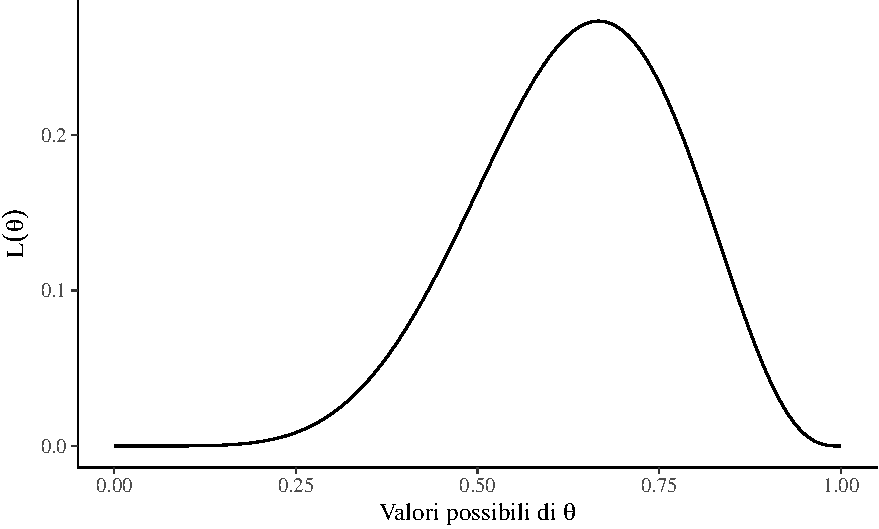
\includegraphics{024_likelihood_files/figure-latex/unnamed-chunk-3-1} \end{center}

Nella simulazione, il valore \(\theta\) che massimizza la funzione di verosimiglianza può essere trovato nel modo seguente:

\begin{Shaded}
\begin{Highlighting}[]
\NormalTok{theta[}\FunctionTok{which.max}\NormalTok{(like)]}
\CommentTok{\#\textgreater{} [1] 0.6666667}
\end{Highlighting}
\end{Shaded}

\noindent
Il valore così trovato è uguale al valore definito dalla \eqref{eq:mlprop}.

\hypertarget{la-verosimiglianza-del-modello-normale}{%
\section{La verosimiglianza del modello Normale}\label{la-verosimiglianza-del-modello-normale}}

Ora che abbiamo capito come costruire la funzione verosimiglianza di
una binomiale è relativamente semplice fare un passo ulteriore e
considerare la verosimiglianza del caso di una funzione di densità,
ovvero nel caso di una variabile casuale continua. Consideriamo qui il
caso della Normale.

La densità di una distribuzione Normale di parametri \(\mu\) e \(\sigma\) è

\[
f(y \mid \mu, \sigma) = \frac{1}{\sigma \sqrt{2\pi}} \exp\left\{-\frac{1}{2\sigma^2}(y-\mu)^2\right\}.
\label{eq:gausslike}
\]

Poniamoci ora il problema di trovare la s.m.v. dei parametri sconosciuti \(\mu\) e \(\sigma\) nel caso in cui le \(n\) osservazioni \(y = (y_1, \dots, y_n)\) sono realizzazioni indipendenti ed identicamente distribuite (di seguito, i.i.d.) della medesima variabile casuale \(Y \sim \mathcal{N}(\mu, \sigma)\). Per semplicità, scriveremo \(\theta = \{\mu, \sigma\}.\)

Il campione osservato è un insieme di eventi, ciascuno dei quali corrisponde alla realizzazione di una variabile casuale --- possiamo pensare ad uno di tali eventi come all'estrazione casuale di un valore dalla ``popolazione'' \(\mathcal{N}(\mu, \sigma)\). Se le variabili casuali sono i.i.d., la loro densità congiunta è data da:

\begin{align}
f(y \mid \theta) &= f(y_1 \mid \theta) \cdot f(y_2 \mid \theta) \cdot \; \dots \; \cdot f(y_n \mid \theta)\notag\\
                 &= \prod_{i=1}^n f(y_i \mid \theta),
\label{eq:gauss-prob-cong}
\end{align}
\noindent
laddove la funzione \(f(\cdot)\) è la \eqref{eq:gausslike}. Tenendo costanti i dati \(y\), la funzione di verosimiglianza è:

\begin{equation}
\mathcal{L}(\theta \mid y) = \prod_{i=1}^n f(y_i \mid \theta).
\label{eq:gausslike2}
\end{equation}

L'obiettivo è quello di massimizzare la funzione di verosimiglianza per trovare i valori \(\theta\) ottimali. Usando la notazione matematica questo si esprime dicendo che cerchiamo l'argmax della \eqref{eq:gausslike2} rispetto a \(\theta\), ovvero

\[
\hat{\theta} = \text{argmax}_{\theta} \prod_{i=1}^n f(y_i \mid \theta).
\]

Questo problema si risolve calcolando le derivate della funzione rispetto a \(\theta\), ponendo le derivate uguali a zero e risolvendo. Saltando tutti i passaggi algebrici di questo procedimento, per \(\mu\) troviamo

\begin{equation}
\hat{\mu} = \frac{1}{n} \sum_{i=1}^n y_i
\label{eq:maxlikemu}
\end{equation}
e per \(\sigma\) abbiamo

\begin{equation}
\hat{\sigma} = \sqrt{\sum_{i=1}^n\frac{1}{n}(y_i- \mu)^2}.
\label{eq:maxlikesigma}
\end{equation}
In altri termini, la s.m.v. del parametro \(\mu\) è la media del campione e la s.m.v. del parametro \(\sigma\) è la deviazione standard del campione.

\hypertarget{simulazione}{%
\subsection{Simulazione}\label{simulazione}}

Consideriamo ora un esempio che utilizza dei dati reali. I dati corrispondono ai valori BDI-II dei trenta soggetti del campione clinico di \citet{zetschefuture2019}:

\begin{Shaded}
\begin{Highlighting}[]
\NormalTok{d }\OtherTok{\textless{}{-}} \FunctionTok{tibble}\NormalTok{(}
  \AttributeTok{y =} \FunctionTok{c}\NormalTok{(}\DecValTok{26}\NormalTok{, }\DecValTok{35}\NormalTok{, }\DecValTok{30}\NormalTok{, }\DecValTok{25}\NormalTok{, }\DecValTok{44}\NormalTok{, }\DecValTok{30}\NormalTok{, }\DecValTok{33}\NormalTok{, }\DecValTok{43}\NormalTok{, }\DecValTok{22}\NormalTok{, }\DecValTok{43}\NormalTok{, }\DecValTok{24}\NormalTok{, }
        \DecValTok{19}\NormalTok{, }\DecValTok{39}\NormalTok{, }\DecValTok{31}\NormalTok{, }\DecValTok{25}\NormalTok{, }\DecValTok{28}\NormalTok{, }\DecValTok{35}\NormalTok{, }\DecValTok{30}\NormalTok{, }\DecValTok{26}\NormalTok{, }\DecValTok{31}\NormalTok{, }\DecValTok{41}\NormalTok{, }\DecValTok{36}\NormalTok{, }
        \DecValTok{26}\NormalTok{, }\DecValTok{35}\NormalTok{, }\DecValTok{33}\NormalTok{, }\DecValTok{28}\NormalTok{, }\DecValTok{27}\NormalTok{, }\DecValTok{34}\NormalTok{, }\DecValTok{27}\NormalTok{, }\DecValTok{22}\NormalTok{)}
\NormalTok{  )}
\end{Highlighting}
\end{Shaded}

Ci poniamo l'obiettivo di creare la funzione di verosimiglianza per questi dati, supponendo, in base ai risultati di ricerche precedenti, di sapere che i punteggi BDI-II si distribuiscono secondo una legge Normale.

Per semplificare il problema, assumeremo di conoscere \(\sigma\) (lo porremo uguale alla deviazione standard del campione) in modo da avere un solo parametro sconosciuto, cioè \(\mu\). Il problema è dunque quello di trovare la funzione di verosimiglianza per il parametro \(\mu\), date le 30 osservazioni del campione e dato \(\sigma = s = 6.61\).

Per una singola osservazione, la funzione di verosimiglianza è la densità Normale espressa in funzione dei parametri. Per un campione di osservazioni i.i.d., ovvero \(y = (y_1, y_2, \dots, y_n)\), la verosimiglianza è la funzione di densità congiunta \(f(y \mid \mu, \sigma)\) espressa in funzione dei parametri, ovvero \(\mathcal{L}(\mu, \sigma \mid y)\). Dato che le osservazioni sono i.i.d., la densità congiunta è data dal prodotto delle densità delle singole osservazioni.

Per semplicità, assumiamo \(\sigma\) noto e uguale alla deviazione standard del campione:

\begin{Shaded}
\begin{Highlighting}[]
\NormalTok{true\_sigma }\OtherTok{\textless{}{-}} \FunctionTok{sd}\NormalTok{(d}\SpecialCharTok{$}\NormalTok{y)}
\NormalTok{true\_sigma }
\CommentTok{\#\textgreater{} [1] 6.606858}
\end{Highlighting}
\end{Shaded}

Avendo posto \(\sigma = 6.61\), per una singola osservazione \(y_i\) abbiamo

\[
f(y_i \mid \mu, \sigma) = \frac{1}{{6.61 \sqrt {2\pi}}}\exp\left\{{-\frac{(y_i - \mu)^2}{2\cdot 6.61^2}}\right\},\notag
\]
dove il pedice \(i\) specifica l'osservazione \(y_i\) tra le molteplici osservazioni \(y\), e \(\mu\) è il parametro sconosciuto che deve essere determinato (nell'esempio, \(\sigma = s\)). La densità congiunta è dunque

\[
f(y \mid \mu, \sigma) = \, \prod_{i=1}^n f(y_i \mid \mu, \sigma)\notag
\]
e, alla luce dei dati osservati, la verosimiglianza diventa

\[
\begin{aligned}
\mathcal{L}(\mu, \sigma \mid y) =& \, \prod_{i=1}^n f(y_i \mid \mu, \sigma) = \notag\\
& \frac{1}{{6.61 \sqrt {2\pi}}}\exp\left\{{-\frac{(26 - \mu)^2}{2\cdot 6.61^2}}\right\} \times \notag\\
 & \frac{1}{{6.61 \sqrt {2\pi}}}\exp\left\{{-\frac{(35 - \mu)^2}{2\cdot 6.61^2}}\right\} \times  \notag\\
& \vdots \notag\\
 & \frac{1}{{6.61 \sqrt {2\pi}}}\exp\left\{{-\frac{(22 - \mu)^2}{2\cdot 6.61^2}}\right\}.
\end{aligned}
\label{eq:lldepression}
\]

Poniamoci ora il problema di rappresentare graficamente la funzione di verosimiglianza per il parametro \(\mu\). Avendo un solo parametro sconosciuto, possiamo rappresentare la verosimiglianza con una curva. In \R, definiamo la funzione di log-verosimiglianza nel modo seguente:

\begin{Shaded}
\begin{Highlighting}[]
\NormalTok{log\_likelihood }\OtherTok{\textless{}{-}} \ControlFlowTok{function}\NormalTok{(y, mu, }\AttributeTok{sigma =}\NormalTok{ true\_sigma) \{}
  \FunctionTok{sum}\NormalTok{(}\FunctionTok{dnorm}\NormalTok{(y, mu, sigma, }\AttributeTok{log =} \ConstantTok{TRUE}\NormalTok{))}
\NormalTok{\}}
\end{Highlighting}
\end{Shaded}

Nella funzione \texttt{log\_likelihood()}, \texttt{y} è un vettore che, nel caso presente contiene \(n = 30\) valori. Per ciascuno di questi valori, la funzione \texttt{dnorm()} trova la densità Normale utilizzando il valore \(\mu\) che passato a \texttt{log\_likelihood()} e il valore \(\sigma\) uguale a 6.61 --- nell'esempio, questo parametro viene assunto come noto. L'argomento \texttt{log\ =\ TRUE} specifica che deve essere preso il logaritmo. La funzione \texttt{dnorm()} è un argomento della funzione \texttt{sum()}. Ciò significa che i 30 valori così trovati, espressi su scala logaritmica, verranno sommati --- sommare logaritmi è equivalente a fare il prodotto dei valori sulla scala originaria.

Se applichiamo questa funzione ad un solo valore \(\mu\) otteniamo l'ordinata della funzione di log-verosimiglianza in corrispondenza del valore \(\mu\) (si veda la figura \eqref{eq:lldepression}). Si noti che, per trovare un tale valore, abbiamo utilizzato le seguenti informazioni:

\begin{itemize}
\tightlist
\item
  i 30 dati del campione,
\item
  il valore \(\sigma = s\) fissato a 6.61,
\item
  il singolo valore \(\mu\) passato alla funzione \texttt{log\_likelihood()}.
\end{itemize}

Avendo trovato un singolo punto della funzione di log-verosimiglianza, dobbiamo ripetere i calcoli precedenti per tutti i possibili valori che \(\mu\) può assumere.

Nel seguente ciclo \texttt{for()} viene calcolata la log-verosimiglianza di 100,000 valori possibili del parametro \(\mu\):

\begin{Shaded}
\begin{Highlighting}[]
\NormalTok{nrep }\OtherTok{\textless{}{-}} \FloatTok{1e5}
\NormalTok{mu }\OtherTok{\textless{}{-}} \FunctionTok{seq}\NormalTok{(}
  \FunctionTok{mean}\NormalTok{(d}\SpecialCharTok{$}\NormalTok{y) }\SpecialCharTok{{-}} \FunctionTok{sd}\NormalTok{(d}\SpecialCharTok{$}\NormalTok{y), }
  \FunctionTok{mean}\NormalTok{(d}\SpecialCharTok{$}\NormalTok{y) }\SpecialCharTok{+} \FunctionTok{sd}\NormalTok{(d}\SpecialCharTok{$}\NormalTok{y), }
  \AttributeTok{length.out =}\NormalTok{ nrep}
\NormalTok{)}

\NormalTok{ll }\OtherTok{\textless{}{-}} \FunctionTok{rep}\NormalTok{(}\ConstantTok{NA}\NormalTok{, nrep)}
\ControlFlowTok{for}\NormalTok{ (i }\ControlFlowTok{in} \DecValTok{1}\SpecialCharTok{:}\NormalTok{nrep) \{}
\NormalTok{  ll[i] }\OtherTok{\textless{}{-}} \FunctionTok{log\_likelihood}\NormalTok{(d}\SpecialCharTok{$}\NormalTok{y, mu[i], true\_sigma)}
\NormalTok{\}}
\end{Highlighting}
\end{Shaded}

Il vettore \texttt{mu} contiene 100,000 possibili valori del parametro \(\mu\); tali valori sono stati scelti nell'intervallo \(\bar{y} \pm s\). Per ciascuno di questi valori la funzione \texttt{log\_likelihood()} calcola il valore di log-verosimiglianza. I 100,000 risultati vengono salvati nel vettore \texttt{ll}.

I vettori \texttt{mu} e \texttt{ll} possono dunque essere usati per disegnare il grafico della funzione di log-verosimiglianza per il parametro \(\mu\):

\begin{Shaded}
\begin{Highlighting}[]
\FunctionTok{tibble}\NormalTok{(mu, ll) }\SpecialCharTok{\%\textgreater{}\%} 
\FunctionTok{ggplot}\NormalTok{(}\FunctionTok{aes}\NormalTok{(}\AttributeTok{x =}\NormalTok{ mu, }\AttributeTok{y =}\NormalTok{ ll)) }\SpecialCharTok{+}
  \FunctionTok{geom\_line}\NormalTok{() }\SpecialCharTok{+}
  \FunctionTok{vline\_at}\NormalTok{(}\FunctionTok{mean}\NormalTok{(d}\SpecialCharTok{$}\NormalTok{y), }\AttributeTok{color =} \StringTok{"sky blue"}\NormalTok{, }\AttributeTok{linetype =} \StringTok{"dashed"}\NormalTok{) }\SpecialCharTok{+}
  \FunctionTok{labs}\NormalTok{(}
    \AttributeTok{y =} \StringTok{"Log{-}verosimiglianza"}\NormalTok{,}
    \AttributeTok{x =} \FunctionTok{expression}\NormalTok{(}\StringTok{"Parametro"}\SpecialCharTok{\textasciitilde{}}\NormalTok{mu)}
\NormalTok{  ) }
\end{Highlighting}
\end{Shaded}

\begin{center}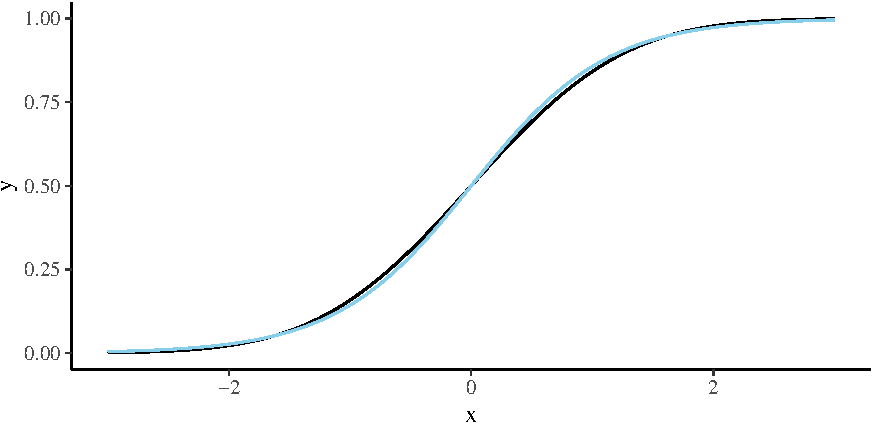
\includegraphics{024_likelihood_files/figure-latex/unnamed-chunk-9-1} \end{center}

Dalla figura notiamo che, per i dati osservati, il massimo della funzione di log-verosimiglianza calcolata per via numerica, ovvero 30.93, è identico alla media dei dati campionari e corrisponde al risultato teorico della \eqref{eq:lldepression}.

\hypertarget{considerazioni-conclusive}{%
\section*{Considerazioni conclusive}\label{considerazioni-conclusive}}
\addcontentsline{toc}{section}{Considerazioni conclusive}

La verosimiglianza viene utilizzata sia nell'inferenza bayesiana che in quella frequentista. In entrambi i paradigmi di inferenza, il suo ruolo è quantificare la forza con la quale i dati osservati supportano i possibili valori dei parametri sconosciuti.

Nella funzione di verosimiglianza i dati (osservati) vengono trattati come fissi, mentre i valori del parametro (o dei parametri) \(\theta\) vengono variati: la verosimiglianza è una funzione di \(\theta\) per il dato fisso \(y\). Pertanto, la funzione di verosimiglianza riassume i seguenti elementi: un modello statistico che genera stocasticamente i dati (in questo capitolo abbiamo esaminato due modelli statistici: quello binomiale e quello Normale), un intervallo di valori possibili per \(\theta\) e i dati osservati \(y\).

Nella statistica frequentista l'inferenza si basa solo sui dati a disposizione e qualunque informazione fornita dalle conoscenze precedenti non viene presa in considerazione. Nello specifico, nella statistica frequentista l'inferenza viene condotta massimizzando la funzione di (log) verosimiglianza, condizionatamente ai valori assunti dalle variabili casuali campionarie. Nella statistica bayesiana, invece, l'inferenza statistica viene condotta combinando la funzione di verosimiglianza con le distribuzioni a priori dei parametri incogniti \(\theta\).

La differenza fondamentale tra inferenza bayesiana e frequentista è dunque che i frequentisti non ritengono utile descrivere in termini probabilistici i parametri: i parametri dei modelli statistici vengono concepiti come fissi ma sconosciuti. Nell'inferenza bayesiana, invece, i parametri sconosciuti sono intesi come delle variabili casuali e ciò consente di quantificare in termini probabilistici il nostro grado di intertezza relativamente al loro valore.

  \bibliography{refs.bib,book.bib,packages.bib}

\end{document}
